\documentclass[tikz, preview]{standalone}

\usepackage{amsfonts, amsthm, amssymb, amsmath, stmaryrd, etoolbox}
\usepackage{tikz}
\usetikzlibrary{matrix,arrows}

\begin{document}
\[
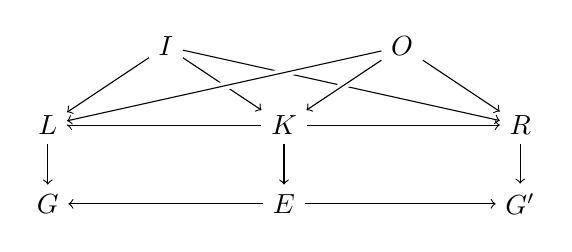
\begin{tikzpicture}
\node (I) at (1.5,2) {$I$};
\node (O) at (4.5,2) {$O$};
\node (L) at (0,1) {$L$};
\node (K) at (3,1) {$K$};
\node (R) at (6,1) {$R$};
\node (G) at (0,0) {$G$};
\node (E) at (3,0) {$E$};
\node (G') at (6,0) {$G'$};
%
\draw [->] (I) edge (L);
\draw [->] (I) edge (K);
\draw [->] (I) edge (R);
\draw [->] (K) edge (L);
\draw [->] (K) edge (E);
\draw [->] (K) edge (R);
\draw [->] (L) edge (G);
\draw [->] (R) edge (G');
\draw [->] (E) edge (G);
\draw [->] (E) edge (G');
%
\draw [-] (O) edge[white,line width=3pt] (L);
\draw [->] (O) edge (L);
\draw [-] (O) edge[white,line width=3pt] (K);
\draw [->] (O) edge (K);
\draw [-] (O) edge[white,line width=3pt] (R);
\draw [->] (O) edge (R);
\end{tikzpicture}
\]
\end{document}
